\question 若8位信息位为11011100,生成多项式G(x)=x\^{}5+x\^{}4+x+1,则生成的CRC码为
\par\fourch{1101 1100 0010 0}{1101 1100 0000 0}{\textcolor{red}{1101 1100 0001 0}}{1001 1100 0000 0}
\begin{solution}C。 设C(x)为信息多项式,G(x)为生成多项式。 CRC码的生成步骤如下:
①将x的最高幂次为R的生成多项式G(x)转换成对应的R+1位二进制数。
②将信息码左移R位,相当与对应的信息多项式C(x)*(2\^{}R)。
③用生成多项式(二进制数)对信息码做除,得到R位的余数。
④将余数拼到信息码左移后空出的位置,得到完整的CRC码。 有效信息M(x)=1101
1100,可知n=8; 由G(x)=110011,由于G(x)为k+1位,可知k=5;
故将有效信息左移5位后再被G(x)模2除,即1101 1100 0000 0。
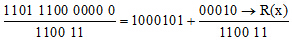
\includegraphics[width=3.04167in,height=0.41667in]{computerassets/37425042f260ca5a3767b94bc041794b.jpeg}
所以M(x)*(x\^{}5)+R(x)=1101 1100 0001 0即为CRC码。
总的信息位为13位,有效信息位为8位,冗余位(检测位)为5位。
\end{solution}
\question 下列属于奇偶校验码特征的是( )。 \ding{192}.只能检查出奇数个比特错误
\ding{193}.能查出任意一个比特位的错误 \ding{194}.比CRC可靠
\par\twoch{仅\ding{192}、\ding{193}}{仅\ding{192}、\ding{194}}{\textcolor{red}{仅\ding{192}}}{仅\ding{193}}
\begin{solution}\ding{192}:奇偶校验的原理是通过增加冗余位来使得码字中``1''的个数保持为奇数个或者偶数个的编码方法。若出现奇数个比特的错误,``1''的个数将与原来``1''的个数不一样,故可以发现奇数个比特的错误。而如果出现偶数个比特的错误,``1''的个数仍然与原来的``1''的个数相同,故无法发现偶数个比特的错误。
\ding{193}:由\ding{192}的分析知\ding{193}错误。
\ding{194}:CRC可以检验出任意位错误,而奇偶校验码只能检验奇数个错误,故\ding{194}错误。
\end{solution}
\question 下列属于奇偶校验码特征的是
\par\twoch{\textcolor{red}{只能检查出奇数个比特错误}}{能查出长度任意一个比特的错误}{比CRC校验可靠}{可以检查偶数个比特的错误}
\begin{solution}奇偶校验的原理是通过增加冗余位来使得码字中``1''的个数保持为奇数个或者偶数个的编码方法。它只能发现奇数个比特的错误。
\end{solution}
\question (北京理工大学)接收端发现有差错时,设法通知发送端重发,直到收到正确的码字为止,这种差错控制方法为
\par\twoch{前向纠错}{冗余检验}{混合差错控制}{\textcolor{red}{自动重发请求}}
\begin{solution}差错控制主要解决错误检测和重发方法。通常可以采用两种方法:一种是前向纠错,即接收端收到有差错的数据帧时,能够自动将差错改正过来,另一种是差错检测,即接收端发现有差错时,设法通知发送端重发,直到收到正确的码字为止,这种方法也称为自动重发请求(ARQ法)。
\end{solution}
